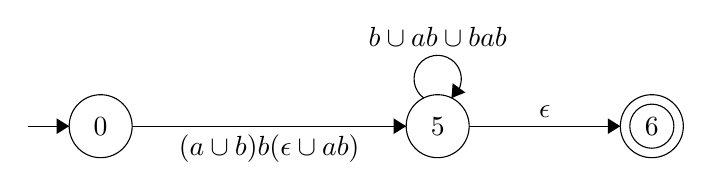
\begin{tikzpicture}[scale=0.2]
    \tikzstyle{every node}+=[inner sep=0pt]
    \draw [black] (4.8,-6.9) circle (2);
    \draw (4.8,-6.9) node {$0$};
    \draw [black] (26.2,-6.9) circle (2);
    \draw (26.2,-6.9) node {$5$};
    \draw [black] (39.8,-6.9) circle (2);
    \draw (39.8,-6.9) node {$6$};
    \draw [black] (39.8,-6.9) circle (1.4);
    \draw [black] (0.2,-6.9) -- (2.8,-6.9);
    \fill [black] (2.8,-6.9) -- (2,-6.4) -- (2,-7.4);
    \draw [black] (28.2,-6.9) -- (37.8,-6.9);
    \fill [black] (37.8,-6.9) -- (37,-6.4) -- (37,-7.4);
    \draw (33,-6.4) node [above] {$\epsilon$};
    \draw [black] (25.318,-5.114) arc (234:-54:1.5);
    \draw (26.2,-1.9) node [above] {$b\cup ab\cup bab$};
    \fill [black] (27.08,-5.11) -- (27.96,-4.76) -- (27.15,-4.17);
    \draw [black] (6.8,-6.9) -- (24.2,-6.9);
    \fill [black] (24.2,-6.9) -- (23.4,-6.4) -- (23.4,-7.4);
    \draw (15.5,-7.4) node [below] {$(a\cup b)b(\epsilon\cup ab)$};
    \end{tikzpicture}